\section{Conventional \ac{1D} Datasets}
\label{sec:evaluation}

As mentioned in \cref{subsec:phase-variance}, one of the disadvantages of
\ac{SVD}-based methods like the \ac{MPM} is their propensity to generate
parameter estimates featuring oscillators with spurious phase behaviour. Such
behaviour is most prevalent in \acp{FID} which (a) feature signals with very
similar frequencies and (b) that have a low \ac{SNR}.
To assess the effectiveness of including the phase variance-regularised
\ac{NLP} routine, comparisons are now made with results generated with the
\ac{MPM} in isolation.

For the experimental datasets considered (\cref{subsec:andro,subsec:cyclo}),
the data was pre-processed using \textsc{Bruker}'s \textsc{TopSpin} software,
using the series of commands \texttt{ft; pk; abs}; these perform \ac{FT},
automatic phase correction, and baseline correction, respectively. The data was
then converted back to the time-domain using \ac{IFT} prior to filtering and
estimation.

\subsection{``Twenty Signals''}
%%% Previously had this as landscape:
% \begin{sidewaysfigure}
%     \centering
%     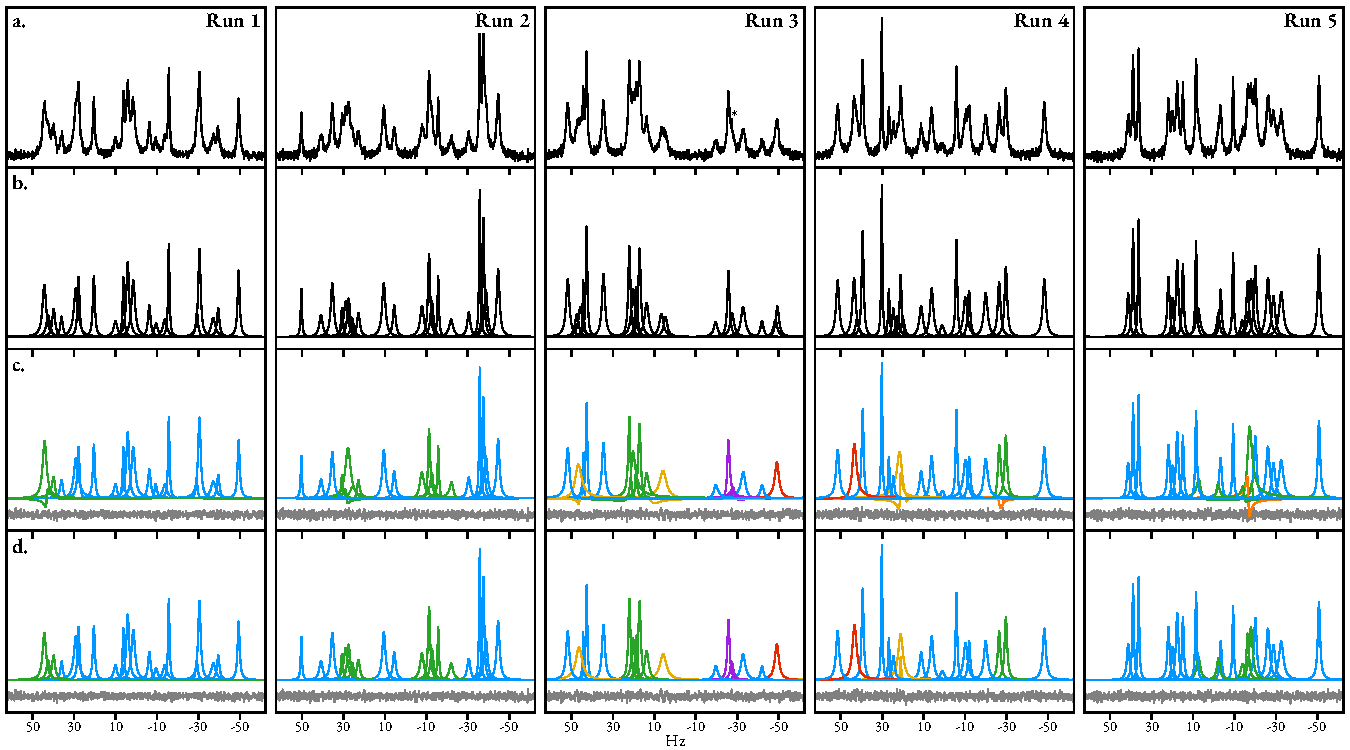
\includegraphics{mpm_vs_nlp/mpm_vs_nlp_landscape.pdf}
%     \caption[
%         The result of estimating a series of 5 simulated \acsp{FID}
%         using both the \acs{MPM} in isolation, and also with phase
%         variance-regularised \acs{NLP} used afterwards.
%     ]{
%         The result of estimating a series of 5 simulated \acp{FID} comprising
%         20 signals. See the main text for details on how the \acp{FID} were
%         constructed.
%         \textbf{a.} Spectra of the \acp{FID} generated.
%         \textbf{b.} Spectral lines corresponding to the set of signals
%         used to generate each \ac{FID}.
%         \textbf{c.} Plots of peaks for each oscillator generated using
%         the \acs{MPM}.
%         \textbf{d.} An equivalent plot for the result after applying phase
%         variance-regularised \acs{NLP}, using the \acs{MPM} result as an
%         initial guess.  Also included in c and d are the
%         residual between the data and the estimated model (grey
%         line). The colouring of the oscillators in c and d is described
%         in the main text.
%     }
%     \label{fig:mpm_vs_nlp}
% \end{sidewaysfigure}
\begin{figure}
    \centering
    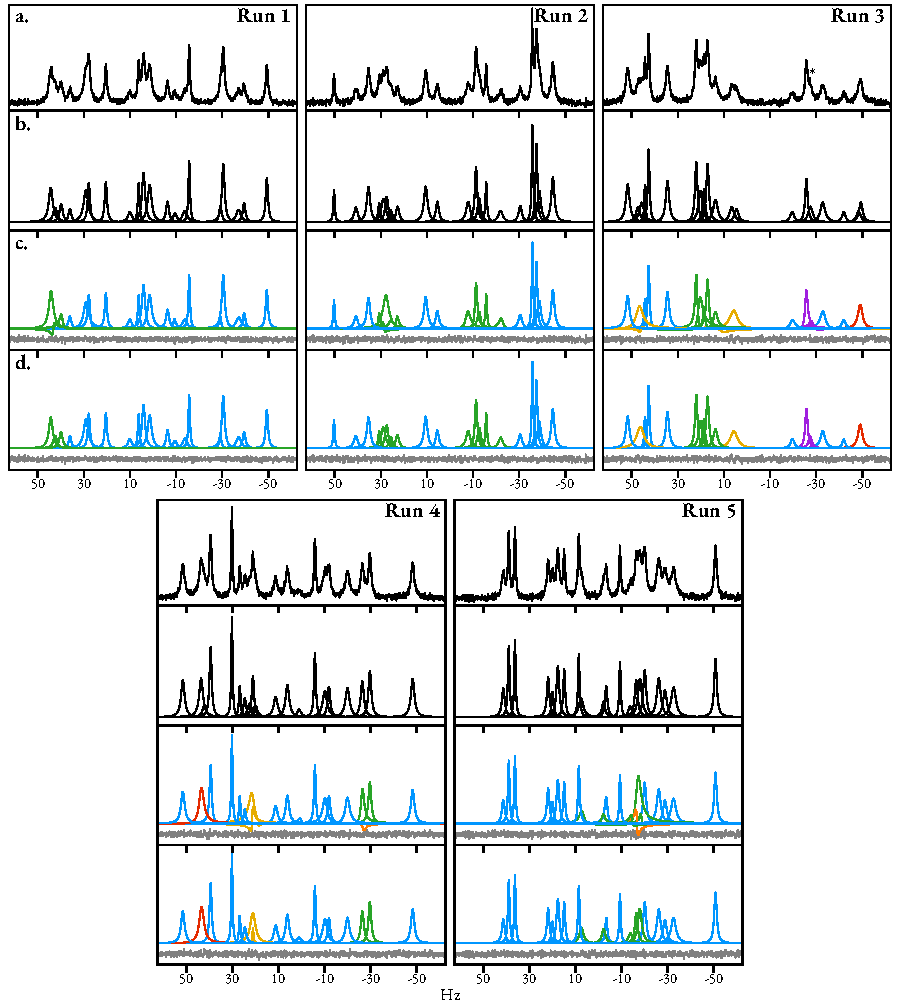
\includegraphics{mpm_vs_nlp/mpm_vs_nlp_portrait.pdf}
    \caption[
        The result of estimating a series of 5 simulated \acsp{FID}
        using both the \acs{MPM} in isolation, and also with phase
        variance-regularised \acs{NLP} used afterwards.
    ]{
        The result of estimating a series of 5 simulated \acp{FID} comprising
        20 signals. See the main text for details on how the \acp{FID} were
        constructed.
        \textbf{a.} Spectra of the \acp{FID} generated.
        \textbf{b.} Spectral lines corresponding to the set of signals
        used to generate each \ac{FID}.
        \textbf{c.} Plots of peaks for each oscillator generated using
        the \acs{MPM}.
        \textbf{d.} An equivalent plot for the result after applying phase
        variance-regularised \acs{NLP}, using the \acs{MPM} result as an
        initial guess.  Also included in c and d are the
        residual between the data and the estimated model (grey
        line).
        Blue oscillators are those produced by the \ac{MPM} which closely agree
        with a true signal.
        Green oscillators are affected notably by the \ac{NLP} routine,
        and end up in good agreement with a true signal.
        Orange oscillators were excessive oscillators generated by the
        \ac{MPM}, which were removed during the \ac{NLP} routine, leading to a
        parsimonious fit of the remaining (green) oscillators in the frequency
        neighbourhood.
        Yellow oscillators denote cases where the number of oscillators produced
        by the \ac{MPM} matched the number of true signals in a given frequency
        neighbourhood. However one of the oscillators was removed during the
        \ac{NLP} routine, leading to an under-fit of the neighbourhood.
        Red oscillators denote an under-fit of a frequency neighbourhood by
        the \ac{MPM}.
        Purple oscillators denote an over-fit of a frequency neighbourhood
        by the \ac{MPM}, with none of the oscillators being removed during
        \ac{NLP} (\textit{cf.} orange oscillators which are removed during
        \ac{NLP}).
    }
    \label{fig:mpm_vs_nlp}
\end{figure}
A series of five simulated \acp{FID} were constructed using
\cref{eq:hypercomplex-fid} with $D=1$. For each \ac{FID}, a model order
of $M=20$ was used, the number of points sampled was $N = 1024$, the sweep
width was $\fsw=\qty{125}{\hertz}$, and the transmitter offset was $\foff
= \qty{0}{\hertz}$.  Each oscillator was assigned a phase of \ang{0}, while the
amplitudes, frequencies and damping factors were drawn at random from the
following distributions
$\forall m \in \lbrace 1, \cdots, 20\rbrace$:
$a_m \sim \mathcal{U}(1, 5)$, $f_m \sim \mathcal{U}(\qty{-55}{\hertz},
\qty{55}{\hertz})$, $\eta_m \sim \mathcal{U}(\qty{2}{\per\second},
\qty{8}{\per\second})$. The frequencies were subjected to an additional
constraint; no two signals were permitted to have frequencies that
differed by less than $\nicefrac{4 \fsw}{N} \approx \qty{0.49}{\hertz}$.
Each noiseless \ac{FID} $\bx$ was then corrupted with \ac{AWGN}, with a target
\ac{SNR} of \qty{25}{\deci\bel}, such that the desired noise variance for each
\ac{FID} was given by (\emph{cf.} \cref{eq:snr,eq:snr-db}):
\begin{equation}
    \sigma^2 = \frac{1}{20^{2.5} \times 1024}
        \sum_{n=0}^{1023} \lvert x_n \rvert^2.
\end{equation}
The spectra of the simulated \acp{FID} are presented in
\cref{fig:mpm_vs_nlp}.a, with the set of oscillator peaks which contribute
to the spectrum in \cref{fig:mpm_vs_nlp}.b. With the criteria used to
constructed the datasets, it can be seen they feature signals which often
suffer from severe overlap, with the high noise variance compounding the
opportunity to clearly identify all contributing signals.

For each \ac{FID}, the \ac{MPM} was performed, assuming a model order of
30, constituting a considerable over-fit of oscillators. The \ac{MDL} tended to
produce under-estimates of $M$ when applied to these \acp{FID}, so the
hard-coded value was used instead to ensure sufficient oscillators were given
to the model. The under-estimates were likely due to the
high \ac{SNR} of the signals\,---\,recall the red signal in \cref{fig:mdl}\,---\,in
conjunction with severe signal overlap. When an excessive model order is
provided to the \ac{MPM}, it is typical that oscillators corresponding to the
noise subspace of the data matrix $\Hy$ are characterised by small amplitudes
and/or very small damping factors. For this reason, prior to subjecting the
\ac{MPM} result to \ac{NLP}, oscillators which satisfied $a_m < 0.1$ and/or
$\eta_m < \qty{0.7}{\per\second}$ were removed from the parameter set. The
individual oscillators which make up the \ac{MPM} result after purging spurious
components are displayed in \cref{fig:mpm_vs_nlp}.c, along with the
residual between the data and the estimated model (i.e. the sum of all
oscillator peaks).

The \ac{MPM} consistently generated models which agreed well with the data
in a least squares sense, as as evidenced by the residuals in
\cref{fig:mpm_vs_nlp}.c.
However, it can be seen that in several spectral regions across the datasets,
especially ones that are highly crowded, oscillators possess parameters which
deviate significantly from the true signal parameters used to constructed the
\acp{FID}.
Most notably, individual oscillator phases regularly stray far from \ang{0},
and their associated amplitudes are often considerably different too.
In \cref{fig:mpm_vs_nlp}.c, blue oscillators are those which
are in very close agreement with a particular true signal in the data.
Oscillators with other colours are not in agreement with a true signal,
with the different colourings described shortly.
The desired outcome of the \ac{NLP} routine is for it to adjust the
parameters associated with non-blue oscillators in \cref{fig:mpm_vs_nlp}.c such
that they agree with true signals, while having little to no effect on those of
the blue oscillators. The results after application of \ac{NLP} are provided in
\cref{fig:mpm_vs_nlp}.d.

In discussing the outcome of the routine, it will be helpful to employ the
concept of a \emph{frequency neighbourhood}, a loose term which describes a
small, continuous subset of frequencies within the spectral window. As the
\ac{NLP} routine involves taking small steps
in parameter space over a number of iterations, it is unlikely that an
oscillator which starts off with a frequency far away from a particular
frequency neighbourhood will eventually enter it. As such, in order for the
\ac{NLP} routine to successfully estimate the signals within a given frequency
neighbourhood of the data, sufficient model oscillators need to present within
the neighbourhood in the initial guess.

Cases where the
\ac{MPM} generated enough oscillators for a given frequency neighbourhood,
albeit with parameters which noticeably deviate from the true signals are
coloured either green or yellow. Green oscillators are those which the \ac{NLP} routine
was able to adjust so as to to achieve agreement with true signals;
they indicate improvements to the estimation result in comparison with the \ac{MPM}
in isolation. Conversely, yellow oscillators denote cases where, though
sufficient oscillators existed in the frequency neighbourhood in the initial
guess, the \ac{NLP} routine evolved such that at least one of the oscillators
was driven by the phase variance constraint to acquire a negative amplitude,
leading to it being removed from the parameter set. This typically occurred with
oscillators that had an initial phase which was either $>
\nicefrac{\pi}{2}$\,\unit{\radian}, or $< -\nicefrac{\pi}{2}$\,\unit{\radian}.
Therefore, yellow oscillators indicate cases where the final result
under-fit the dataset.

There are a couple of instances, denoted by red oscillators,
where the \ac{MPM} assigned too few oscillators to a particular frequency
neighbourhood, and as such the \ac{NLP} routine would not have been able to
yield any major improvement. This occurred in what can safely be described as
fiendishly difficult cases, where severe signal overlap and low \ac{SNR} make
it very difficult to associate certain spectral regions with more than one
signal by eye.

The final two oscillator groupings, coloured purple and orange respectively,
indicate scenarios where the \ac{MPM} generated more oscillators than true
signals in a given frequency neighbourhood (i.e. the data was over-fit in these
regions). Orange
oscillators we purged by the \ac{NLP} routine as they acquired negative
amplitudes. This enabled parsimonious fits of the relevant frequency neighbourhoods by
the oscillators which remained, i.e. the green oscillators in close proximity
to the orange ones in \cref{fig:mpm_vs_nlp}.c. Finally, the purple oscillators
denote the one
occasion (Run 3) where an over-fit occurred, and the model order was not
successfully reduced by the \ac{NLP} routine. One of the purple oscillators in
the \ac{MPM} appears to agree closely with a significant ``blip'' in the noise,
denoted by an asterisk in \cref{fig:mpm_vs_nlp}.a.
The over-fit has therefore occurred because this noise component was
incorporated into the final result; it was neither purged based on the
amplitude and damping factor criteria outlined above, nor by acquiring a
negative amplitude during \ac{NLP}.

\subsection{Andrographolide}
\label{subsec:andro}
\begin{sidewaysfigure}
    \centering
    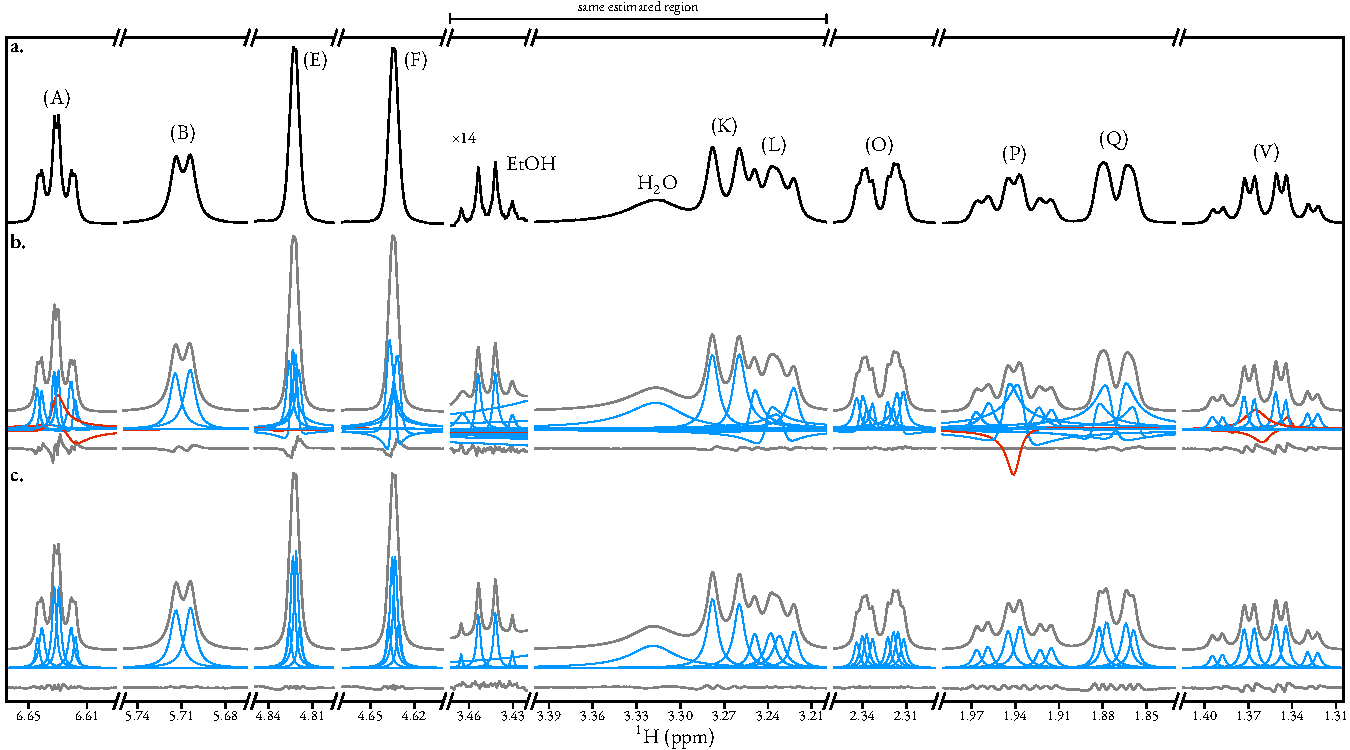
\includegraphics{andrographolide_onedim/andrographolide_onedim.pdf}
    \caption[
        The result of applying the estimation routine to selected regions of a
        pulse-acquire dataset of andrographolide.
    ]{
        The result of applying the estimation routine to selected regions of a
        pulse-acquire dataset of andrographolide in \acs{DMSOd6}.
        \textbf{a.} Spectral regions considered.
        \textbf{b.} The result of applying the \acs{MPM} to the regions, with
        the model order predicted using the \acs{MDL}. Blue and red lines denote
        individual oscillator peaks, while the grey line above is the sum of all
        oscillators. They grey line below is the residual between the data and
        the model.
        \textbf{c.} The result after convergence of the \acs{NLP} routine, again
        with the model above and residual below.
        Red peaks in b correspond to oscillators which acquire negative
        amplitudes and are removed during the \acs{NLP} routine.
        One of the estimated regions has been split in two in the
        figure to save space, with one half, featuring a signal from ethanol,
        being magnified.
    }
    \label{fig:andro-onedim}
\end{sidewaysfigure}
\Cref{fig:andro-onedim} illustrates the outcome of applying the
estimation routine to a \textsuperscript{1}H dataset of
andrographolide (\cref{fig:structures}.a) in \acs{DMSOd6}, acquired with
a \qty{600}{\mega\hertz} spectrometer.
Various spectral regions were chosen for study, and for each one, a
frequency-filtered sub-\ac{FID} was produced using the approach in
\cref{sec:filtering}.
The \ac{MPM} was used to generate an initial guess of parameters, using the
\ac{MDL} to predict the model order in each case. The result of applying the
\ac{MPM} are presented in \cref{fig:andro-onedim}.b. The initial guess
was then subjected to \ac{NLP}, giving rise to the result
\cref{fig:andro-onedim}.c.

The \ac{NLP} routine was effective at resolving the spurious phase behaviour
often generated by the \ac{MPM}.
The estimation method's ability to parametrise signals with high
dynamic range and high variation of damping factors is also evidenced;
a broad intense singlet from water, and a low-intensity quartet from
residual ethanol in the sample, present in the same sub-\ac{FID}, could both
estimated admirably for example.
For some of the sub-\acp{FID} considered, the \ac{MPM} output featured
oscillators, commonly with very high damping factor and/or phases far from
\ang{0}, which were removed during the \ac{NLP} routine (see the red
peaks in panel b). The removal of these, along with the enforcement
of consistent oscillator phases, leads to parameter
estimates which describe the apparent multiplet structures associated with each
spin well. \Cref{tab:andro-multiplets} provides an overview of the
most significant couplings associated with the spins giving rise to the
multiplet structures considered.
\begin{table}
\centering
\begin{tabular}{c c c}
\hline
Spin  & Coupling partners & Multiplet structure \\
\hline
\multicolumn{3}{c}{\textbf{Andrographolide}}\\
\hline
(A) & (D)\textsuperscript{long}, (M)\textsuperscript{vic}, (N)\textsuperscript{vic} & ddd (\emph{dt}) \\
(B) & (D)\textsuperscript{ex} & d \\
(E) & (F)\textsuperscript{vinyl} \dots & d\dots \\
(F) & (E)\textsuperscript{vinyl} \dots & d\dots \\
(K) & (J)\textsuperscript{gem}, (H)\textsuperscript{ex} & d \\
(L) & (C)\textsuperscript{ex}, (T)\textsuperscript{180}, (U)\textsuperscript{60} & dd \\
(O) & (P)\textsuperscript{gem}, (R)\textsuperscript{60}, (V)\textsuperscript{60} & ddd \\
(P) & (O)\textsuperscript{gem}, (R)\textsuperscript{60}, (V)\textsuperscript{180} & ddd (\emph{dt}) \\
(Q) & (M)\textsuperscript{vic}, (N)\textsuperscript{vic} \dots & dd\dots \\
(V) & (O)\textsuperscript{60}, (P)\textsuperscript{180}, (R)\textsuperscript{g}, (W)\textsuperscript{180} & dddd (\emph{dq}) \\
\hline
\multicolumn{3}{c}{\textbf{Cyclosporin A}}\\
\hline
(A) & diastereotopic pair on \textsuperscript{\textbeta}C & dd \\
(B) & ---''--- & dd \\
(C) & ---''--- \& amide proton & ddd (\emph{dt}) \\
(D) & proton on \textsuperscript{\textbeta}C \& amide proton & dd \\
(E) & methyl protons on \textsuperscript{\textbeta}C \& amide proton & dq \\
(F) & ---''--- & dq (\emph{quintet}) \\
\hline
\end{tabular}
\caption[
    The major coupling partners associated with spins in andrographolide and
    cyclosporin A, along with the multiplet structures that arise.
]{
    The major coupling partners associated with spins in andrographolide and
    cyclosporin, considered in \cref{fig:andro-onedim,fig:cyclosporin}
    respectively, along with the multiplet structures that arise.
    For andrographolide, coupling partners are labelled as follows:
    \textsuperscript{vinyl} geminal coupling between two vinylic protons,
    \textsuperscript{ex} geminal coupling between two protons, with one
    bonded to an oxygen, leading to exchange decoupling\cite[Section
    2.6.1.5]{Claridge2016},
    \textsuperscript{gem} geminal coupling between two spins whose dihedral
    angle is not fixed,
    \textsuperscript{long} long-range coupling,
    \textsuperscript{vic} vicinal coupling,
    \textsuperscript{60} geminal coupling, with a fixed dihedral angle of
    \ang{60} between the spins,
    \textsuperscript{180} geminal coupling, with a fixed dihedral angle of
    \ang{180} between the spins.
    All cyclosporin couplings for the spins considered are geminal couplings.
    In cases where the observed multiplet structure is different to the true
    structure, the observed structure is is in brackets. Ellipses denote cases
    where more (long-range) coupling partners are likely, based on the
    estimation result generated/the appearance of the spectrum, though these
    have not been explicitly assigned.
}
\label{tab:andro-multiplets}
\end{table}

One of the most challenging aspects of estimating \ac{NMR} signals is
the common presence of signals within the dataset that have incredibly similar
frequencies due to the influence of scalar couplings.
Molecules with fused ring systems such as andrographolide are prime examples of spin
systems which generate such datasets, as they tend to have very dense coupling
networks leading to complex multiplet structures. Furthermore, fused systems often
exhibit appreciable long-range couplings (between spins separated by four or
more bonds) alongside ubiquitous two-bond (\emph{geminal}) and three-bond
(\emph{vicinal}) couplings. Long range couplings can be particularly challenging to
resolve, as they are often of a comparable magnitude to the spectral resolution
($\nicefrac{\fsw}{N}$), making individual signals barely perceptible.

Take the multiplet structure from spin (Q) as an example of a particularly
challenging estimation problem.
(Q) has separate vicinal couplings to the
diastereotopic protons (M) and (N); these are the couplings to
(Q) of greatest magnitude. If these were the only couplings, a doublet of doublets
(dd) structure would be expected, which is what has been generated by
the estimation routine.
However, a comparison of the data and
the model indicates that there is a clear discrepancy between the two,
evidenced by systematic deviations in the residual; this feature hints at an
under-fit of the data.
% The \ac{MPM} generated oscillators with phases deviating far from \ang{0},
% which enabled good agreement with the data in a residual sense, though of
% course such a set of oscillators is unrealistic in the context of a phased
% \ac{FID}.
Long-range couplings with magnitudes that are large enough to influence the
appearance of (Q)'s multiplet structure are likely to be present, which leads
to frequency neighbourhood in which all contributing signals are too poorly
resolved to realistically gleam any further meaningful information, at least at
the field strength used.

As a second illustration, the multiplet structure corresponding to spin (V) is also
under-fit, this time because the presence of a number of couplings of similar
magnitude leads to resonances coalescing at roughly the same frequency. A
multiplet structure featuring 16 resonances forming in ``dddd'' structure is
expected. However, 3 of the couplings are of similar magnitudes, such that
many of the contributing signals coalesce to form what is apparently a quartet
of doublets (dq).
The estimation routine was able to resolve this dq structure,
however the large deviations in the residual again imply that under-fitting has
occurred, and each oscillator in the parameter set is in fact being used to fit
two or more signals present in the \ac{FID}. Again, at the field strength used
to acquire the \ac{FID}, it is unlikely that an accurate resolution of all 16
signals by estimation is feasible.

% At this point, with two examples provided of cases where poor \ac{RSS} fits
% have resulted, one may question whether the underlying model is actually suited
% to describe the data.
% There is for example precedent for fitting oscillators with non-exponential
% decay profiles\,---\,profiles which lead to Voigt and Gaussian spectral
% lineshapes are common\,---\,to improve the model fit\cite{Sima2007}.
% However, for some multiplet structures in Figure \ref{fig:andro-onedim},
% exceptionally good agreement between the model and data are made, using a
% parsimonious set of parameters.
With three couplings of different magnitude, spin (O) exhibits a ``ddd''
multiplet structure in which all 8 signals are discernible. The \ac{NLP}
routine performed well in taking the initial guess from the
\ac{MPM}\,---\,featuring the correct number of oscillators albeit with
spurious phases\,---\, and generating a well-phased set of oscillators defining
the ddd structure, with a very small associated residual. This highlights that
in cases where all signals present in a given frequency neighbourhood are
resolvable, effective estimation results are achievable.

\subsection{Cyclosporin A}
\label{subsec:cyclo}
\begin{figure}
    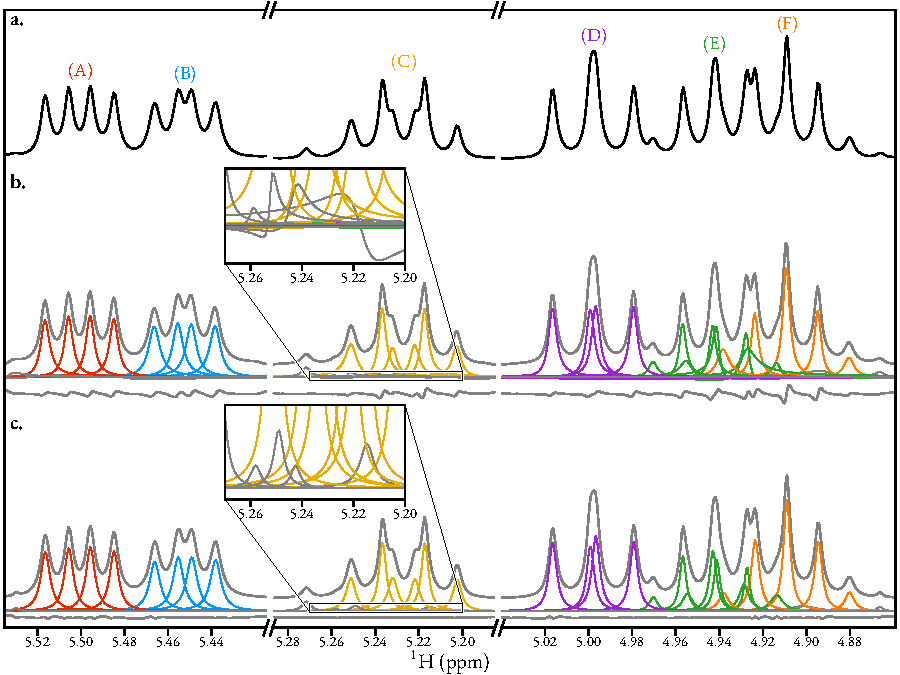
\includegraphics{cyclosporin/cyclosporin.pdf}
    \caption[
        The result of applying the estimation routine to selected regions of a
        pulse-acquire dataset of cyclosporin A.
    ]{
        The result of applying the estimation routine to selected regions of a
        pulse-acquire dataset of cyclosporin A in benzene-d\textsubscript{6}.
        \textbf{a.} The structure of cyclosporin A, with relevant proton
        environments highlighted.
        \textbf{b.} Spectral regions considered.
        \textbf{c.} The result of applying the \acs{MPM} on the regions, with
        the model order predicted using the \acs{MDL}.
        The grey lines above and below the individual oscillator peaks denote
        the sum of all oscillators and the residual between the data and the
        model, respectively.
        \textbf{d.} The result after convergence of the \acs{NLP} routine,
        presented in the same format as panel c.
        Coloured oscillators have been mapped to particular cyclosporin A
        environments. Grey oscillators are not associated with
        cyclosporin A; these are likely due to impurities in the sample.
    }
    \label{fig:cyclosporin}
\end{figure}
The estimation routine was also applied to selected regions of a
\proton\ pulse-acquire dataset of cyclosporin A
(\cref{fig:structures}.b), a cyclic peptide comprising 11 amino
acids, in benzene-d\textsubscript{6}.
The regions considered all comprise
signals arising from protons bound to C\textsuperscript{\textalpha} atoms in
the peptide backbone\cite{Verma2018}.
The estimation procedure used was equivalent to
that used for the andrographolide example.

For the most downfield region
considered, featuring signals from spins (A) and (B), the \ac{MPM} performed
admirably, with the two well-resolved dd multiplet structures present
accurately parametrised by the 8 oscillators in the model; the \ac{NLP} routine
hardly perturbed the initial guess as a result.

In the middle region, which features a doublet of triplets (dt) multiplet structure
from spin (C), low intensity ``shoulders'' are noticeable;
these are likely from low-concentration impurities in the sample. The \ac{MPM}
was able to resolve the dt structure, and characterise
some low intensity signals too, though the phases of these are highly
inconsistent, with a knock-on effect for the relative amplitudes of signals
describing the dt structure (these are expected to abide by the ratio
1:2:1:1:2:1). The \ac{NLP} routine, by enforcing low phase variance in the
oscillators, subtly adjusted the parameter estimate to achieve a set of
oscillator amplitudes that are more consistent with this ratio.

The most downfield region contains three separate multiplet structures
featuring significant signal overlap in the Fourier domain, particularly
involving those corresponding to spins (E) and (F).
The \ac{MPM} produced sufficient oscillators to model these
structures (see \cref{tab:andro-multiplets} for an outline of the structures
present).
However, particularly in the most crowded section around
\SIrange{4.96}{4.92}{\partspermillion} it can be seen that certain oscillators
have phases which noticeably deviate from \ang{0}. In applying the \ac{NLP}
routine, not only did the phases become more consistent,
but the oscillator amplitudes also become more agreeable.
For example, the highest- and lowest-frequency model oscillators
associated with the 1:3:6:3:1 quintet of spin (F) (denoted by
\textdagger\ in Figures \ref{fig:cyclosporin}.b and \ref{fig:cyclosporin}.c)
acquire amplitudes which are much closer in value after \ac{NLP}, as expected.
The most
notable flaw in the final result is associated with the two oscillators marked
by \textdaggerdbl\ in panel c, both of which are associated with the
1:3:1:3:3:1:3:1 dq structure from spin (E). A 1:3 amplitude ratio is expected
between these oscillators. However, in the final \ac{NLP} result, these
had an unexpected ratio of $\approx 1:1$. It is not surprising
that greater deviations from the expected result occur in more heavily crowded spectral
regions, since there is a larger set of values in the parameter space which
will lead to acceptable fits of the data in an \ac{RSS} sense. Nonetheless,
armed simply with knowledge that the data is phased, the routine performs
admirably in highlighting  how the spectrum breaks down into its various
signal components. An improved estimation result could be attained by
supplying the \ac{NLP} routine with more knowledge in the form of parameter
constraints. While this has not been implemented in this work, it is discussed
in \cref{sec:future-work} as a possible pursuit for the future.
